% documentclass: article used for scientific journals, short reports, program documentation, etc
% options: fontsize 11, generate document for double sided printing, a4-paper
\documentclass[11pt, twoside, a4paper]{article}

% package for changing page layout
\usepackage{geometry}
\geometry{a4paper, lmargin=30mm, rmargin=20mm, tmargin=30mm, bmargin=20mm}
% set indentation
\setlength{\parindent}{0mm} 

% input encoding for special characters (e.g. ä,ü,ö,ß), only for non english text
% options: utf8 as encoding standard
\usepackage[utf8]{inputenc}
% package for changing used language
% options: german or default: english
\usepackage[german]{babel}

% package for math symbols, functions and environments from ams(american mathematical society)
\usepackage{amsmath}
% package for extended symbols from ams
\usepackage{amssymb}
% package for extended symbols from stmaryrd(st mary road)
%\usepackage{stmaryrd}
% package for managing pictures
\usepackage{graphicx}

% package for some extra fonts
\usepackage{txfonts}
% package for changing color of font and paper
% options: using names of default colors (e.g red, black)
\usepackage[usenames]{color}

% package for converting eps-files to pdf-files and then include them
\usepackage{epstopdf}
% use another program (ps2pdf) for converting
% !!! important: set shell_escape=1 in /etc/texmf/texmf.cnf (Linux) for allowing to use other programs
% !!!			 or use the command line with -shell-escape
\epstopdfDeclareGraphicsRule{.eps}{pdf}{.pdf}{
ps2pdf -dEPSCrop #1 \OutputFile
}

% package for reference to last page (output number of last page)
\usepackage{lastpage}
% package for using header and footer
% options: automate terms of right and left marks
\usepackage[automark]{scrpage2}
% set style for footer and header
\pagestyle{scrheadings}
% clear pagestyle for redefining
\clearscrheadfoot
% set header and footer: use <xx>head/foot[]{Text} (i...inner, o...outer, c...center, o...odd, e...even, l...left, r...right)
\ihead[]{}
\ohead[]{}
\cfoot[]{\pagemark/\pageref{LastPage}}


% begin the document
\begin{document}
	
	\begin{figure}
		\center
		% GNUPLOT: LaTeX picture with Postscript
\begingroup
  \makeatletter
  \providecommand\color[2][]{%
    \GenericError{(gnuplot) \space\space\space\@spaces}{%
      Package color not loaded in conjunction with
      terminal option `colourtext'%
    }{See the gnuplot documentation for explanation.%
    }{Either use 'blacktext' in gnuplot or load the package
      color.sty in LaTeX.}%
    \renewcommand\color[2][]{}%
  }%
  \providecommand\includegraphics[2][]{%
    \GenericError{(gnuplot) \space\space\space\@spaces}{%
      Package graphicx or graphics not loaded%
    }{See the gnuplot documentation for explanation.%
    }{The gnuplot epslatex terminal needs graphicx.sty or graphics.sty.}%
    \renewcommand\includegraphics[2][]{}%
  }%
  \providecommand\rotatebox[2]{#2}%
  \@ifundefined{ifGPcolor}{%
    \newif\ifGPcolor
    \GPcolorfalse
  }{}%
  \@ifundefined{ifGPblacktext}{%
    \newif\ifGPblacktext
    \GPblacktexttrue
  }{}%
  % define a \g@addto@macro without @ in the name:
  \let\gplgaddtomacro\g@addto@macro
  % define empty templates for all commands taking text:
  \gdef\gplbacktext{}%
  \gdef\gplfronttext{}%
  \makeatother
  \ifGPblacktext
    % no textcolor at all
    \def\colorrgb#1{}%
    \def\colorgray#1{}%
  \else
    % gray or color?
    \ifGPcolor
      \def\colorrgb#1{\color[rgb]{#1}}%
      \def\colorgray#1{\color[gray]{#1}}%
      \expandafter\def\csname LTw\endcsname{\color{white}}%
      \expandafter\def\csname LTb\endcsname{\color{black}}%
      \expandafter\def\csname LTa\endcsname{\color{black}}%
      \expandafter\def\csname LT0\endcsname{\color[rgb]{1,0,0}}%
      \expandafter\def\csname LT1\endcsname{\color[rgb]{0,1,0}}%
      \expandafter\def\csname LT2\endcsname{\color[rgb]{0,0,1}}%
      \expandafter\def\csname LT3\endcsname{\color[rgb]{1,0,1}}%
      \expandafter\def\csname LT4\endcsname{\color[rgb]{0,1,1}}%
      \expandafter\def\csname LT5\endcsname{\color[rgb]{1,1,0}}%
      \expandafter\def\csname LT6\endcsname{\color[rgb]{0,0,0}}%
      \expandafter\def\csname LT7\endcsname{\color[rgb]{1,0.3,0}}%
      \expandafter\def\csname LT8\endcsname{\color[rgb]{0.5,0.5,0.5}}%
    \else
      % gray
      \def\colorrgb#1{\color{black}}%
      \def\colorgray#1{\color[gray]{#1}}%
      \expandafter\def\csname LTw\endcsname{\color{white}}%
      \expandafter\def\csname LTb\endcsname{\color{black}}%
      \expandafter\def\csname LTa\endcsname{\color{black}}%
      \expandafter\def\csname LT0\endcsname{\color{black}}%
      \expandafter\def\csname LT1\endcsname{\color{black}}%
      \expandafter\def\csname LT2\endcsname{\color{black}}%
      \expandafter\def\csname LT3\endcsname{\color{black}}%
      \expandafter\def\csname LT4\endcsname{\color{black}}%
      \expandafter\def\csname LT5\endcsname{\color{black}}%
      \expandafter\def\csname LT6\endcsname{\color{black}}%
      \expandafter\def\csname LT7\endcsname{\color{black}}%
      \expandafter\def\csname LT8\endcsname{\color{black}}%
    \fi
  \fi
  \setlength{\unitlength}{0.0500bp}%
  \begin{picture}(9070.00,11338.00)%
    \gplgaddtomacro\gplbacktext{%
      \csname LTb\endcsname%
      \put(1078,2005){\makebox(0,0)[r]{\strut{}25.00}}%
      \put(1078,4173){\makebox(0,0)[r]{\strut{}30.00}}%
      \put(1078,6341){\makebox(0,0)[r]{\strut{}35.00}}%
      \put(1078,8509){\makebox(0,0)[r]{\strut{}40.00}}%
      \put(1078,10677){\makebox(0,0)[r]{\strut{}45.00}}%
      \put(1210,484){\makebox(0,0){\strut{}0.20}}%
      \put(2358,484){\makebox(0,0){\strut{}0.40}}%
      \put(3506,484){\makebox(0,0){\strut{}0.60}}%
      \put(4654,484){\makebox(0,0){\strut{}0.80}}%
      \put(5803,484){\makebox(0,0){\strut{}1.00}}%
      \put(6951,484){\makebox(0,0){\strut{}1.20}}%
      \put(8099,484){\makebox(0,0){\strut{}1.40}}%
      \put(176,5690){\rotatebox{-270}{\makebox(0,0){\strut{}$p \ [bar]$}}}%
      \put(4941,154){\makebox(0,0){\strut{}$V \ [cm^3]$}}%
      \put(4941,11007){\makebox(0,0){\strut{}Isothermennetz für Schwefelhexafluorid}}%
    }%
    \gplgaddtomacro\gplfronttext{%
      \csname LTb\endcsname%
      \put(7686,10504){\makebox(0,0)[r]{\strut{}$\vartheta \pm \Delta\vartheta = (25.9 \pm 0.1) ^\circ C$}}%
      \csname LTb\endcsname%
      \put(7686,10284){\makebox(0,0)[r]{\strut{}$\vartheta \pm \Delta\vartheta = (40.2 \pm 0.1) ^\circ C$}}%
      \csname LTb\endcsname%
      \put(7686,10064){\makebox(0,0)[r]{\strut{}$\vartheta \pm \Delta\vartheta = (43.9 \pm 0.1) ^\circ C$}}%
      \csname LTb\endcsname%
      \put(7686,9844){\makebox(0,0)[r]{\strut{}$\vartheta \pm \Delta\vartheta = (45.5 \pm 0.1) ^\circ C$}}%
      \csname LTb\endcsname%
      \put(7686,9624){\makebox(0,0)[r]{\strut{}$\vartheta \pm \Delta\vartheta = (50.2 \pm 0.1) ^\circ C$}}%
      \csname LTb\endcsname%
      \put(7686,9404){\makebox(0,0)[r]{\strut{}Isotherme für ideales Gas bei $\vartheta = 45.5 ^\circ C$}}%
    }%
    \gplbacktext
    \put(0,0){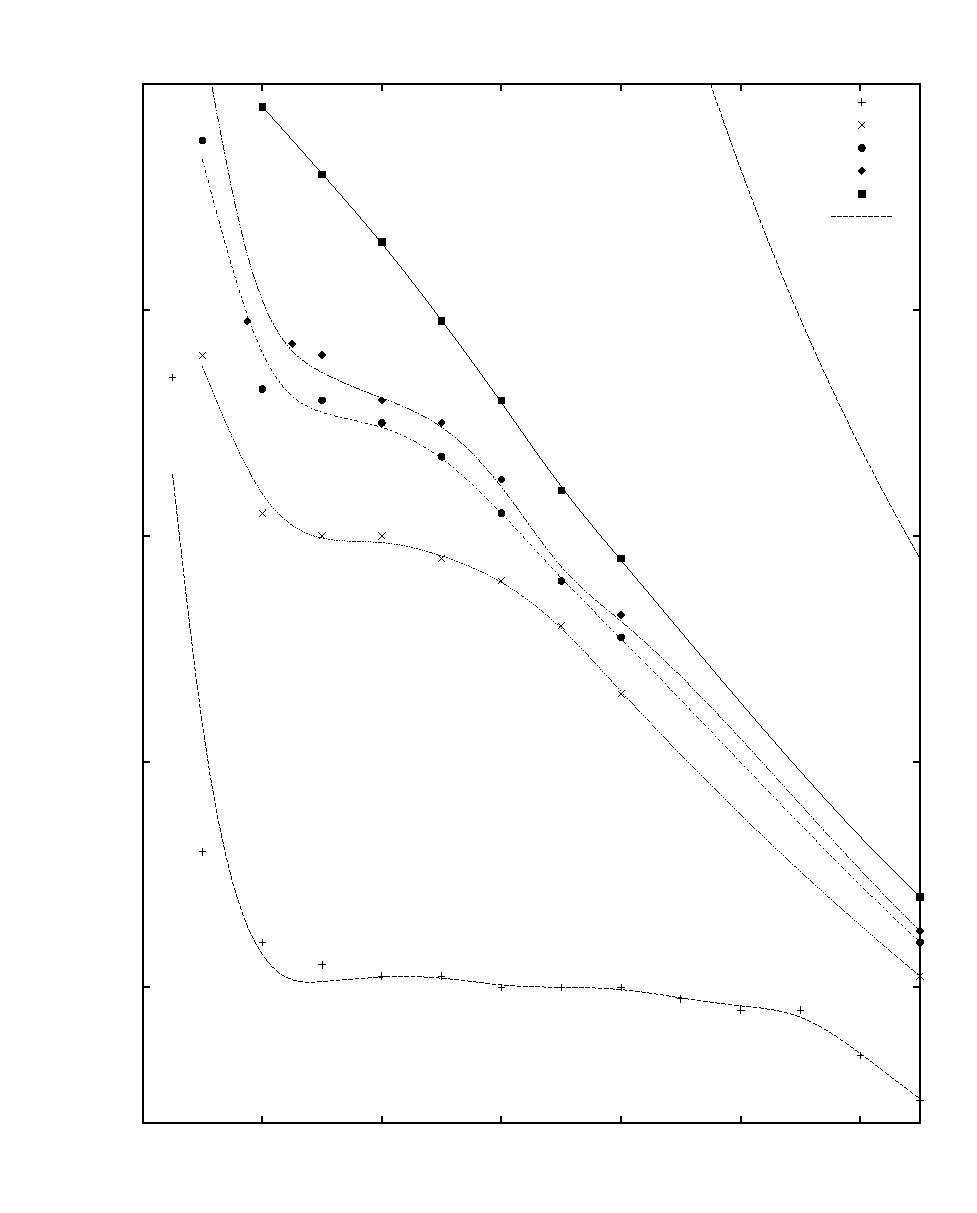
\includegraphics{diagram}}%
    \gplfronttext
  \end{picture}%
\endgroup

	\end{figure}

	\begin{figure}
		\center
		% GNUPLOT: LaTeX picture with Postscript
\begingroup
  \makeatletter
  \providecommand\color[2][]{%
    \GenericError{(gnuplot) \space\space\space\@spaces}{%
      Package color not loaded in conjunction with
      terminal option `colourtext'%
    }{See the gnuplot documentation for explanation.%
    }{Either use 'blacktext' in gnuplot or load the package
      color.sty in LaTeX.}%
    \renewcommand\color[2][]{}%
  }%
  \providecommand\includegraphics[2][]{%
    \GenericError{(gnuplot) \space\space\space\@spaces}{%
      Package graphicx or graphics not loaded%
    }{See the gnuplot documentation for explanation.%
    }{The gnuplot epslatex terminal needs graphicx.sty or graphics.sty.}%
    \renewcommand\includegraphics[2][]{}%
  }%
  \providecommand\rotatebox[2]{#2}%
  \@ifundefined{ifGPcolor}{%
    \newif\ifGPcolor
    \GPcolorfalse
  }{}%
  \@ifundefined{ifGPblacktext}{%
    \newif\ifGPblacktext
    \GPblacktexttrue
  }{}%
  % define a \g@addto@macro without @ in the name:
  \let\gplgaddtomacro\g@addto@macro
  % define empty templates for all commands taking text:
  \gdef\gplbacktext{}%
  \gdef\gplfronttext{}%
  \makeatother
  \ifGPblacktext
    % no textcolor at all
    \def\colorrgb#1{}%
    \def\colorgray#1{}%
  \else
    % gray or color?
    \ifGPcolor
      \def\colorrgb#1{\color[rgb]{#1}}%
      \def\colorgray#1{\color[gray]{#1}}%
      \expandafter\def\csname LTw\endcsname{\color{white}}%
      \expandafter\def\csname LTb\endcsname{\color{black}}%
      \expandafter\def\csname LTa\endcsname{\color{black}}%
      \expandafter\def\csname LT0\endcsname{\color[rgb]{1,0,0}}%
      \expandafter\def\csname LT1\endcsname{\color[rgb]{0,1,0}}%
      \expandafter\def\csname LT2\endcsname{\color[rgb]{0,0,1}}%
      \expandafter\def\csname LT3\endcsname{\color[rgb]{1,0,1}}%
      \expandafter\def\csname LT4\endcsname{\color[rgb]{0,1,1}}%
      \expandafter\def\csname LT5\endcsname{\color[rgb]{1,1,0}}%
      \expandafter\def\csname LT6\endcsname{\color[rgb]{0,0,0}}%
      \expandafter\def\csname LT7\endcsname{\color[rgb]{1,0.3,0}}%
      \expandafter\def\csname LT8\endcsname{\color[rgb]{0.5,0.5,0.5}}%
    \else
      % gray
      \def\colorrgb#1{\color{black}}%
      \def\colorgray#1{\color[gray]{#1}}%
      \expandafter\def\csname LTw\endcsname{\color{white}}%
      \expandafter\def\csname LTb\endcsname{\color{black}}%
      \expandafter\def\csname LTa\endcsname{\color{black}}%
      \expandafter\def\csname LT0\endcsname{\color{black}}%
      \expandafter\def\csname LT1\endcsname{\color{black}}%
      \expandafter\def\csname LT2\endcsname{\color{black}}%
      \expandafter\def\csname LT3\endcsname{\color{black}}%
      \expandafter\def\csname LT4\endcsname{\color{black}}%
      \expandafter\def\csname LT5\endcsname{\color{black}}%
      \expandafter\def\csname LT6\endcsname{\color{black}}%
      \expandafter\def\csname LT7\endcsname{\color{black}}%
      \expandafter\def\csname LT8\endcsname{\color{black}}%
    \fi
  \fi
  \setlength{\unitlength}{0.0500bp}%
  \begin{picture}(8502.00,5102.00)%
    \gplgaddtomacro\gplbacktext{%
      \csname LTb\endcsname%
      \put(682,704){\makebox(0,0)[r]{\strut{}10}}%
      \put(682,1119){\makebox(0,0)[r]{\strut{}15}}%
      \put(682,1534){\makebox(0,0)[r]{\strut{}20}}%
      \put(682,1950){\makebox(0,0)[r]{\strut{}25}}%
      \put(682,2365){\makebox(0,0)[r]{\strut{}30}}%
      \put(682,2780){\makebox(0,0)[r]{\strut{}35}}%
      \put(682,3195){\makebox(0,0)[r]{\strut{}40}}%
      \put(682,3611){\makebox(0,0)[r]{\strut{}45}}%
      \put(682,4026){\makebox(0,0)[r]{\strut{}50}}%
      \put(682,4441){\makebox(0,0)[r]{\strut{}55}}%
      \put(814,484){\makebox(0,0){\strut{}0.0}}%
      \put(1725,484){\makebox(0,0){\strut{}0.5}}%
      \put(2637,484){\makebox(0,0){\strut{}1.0}}%
      \put(3548,484){\makebox(0,0){\strut{}1.5}}%
      \put(4460,484){\makebox(0,0){\strut{}2.0}}%
      \put(5371,484){\makebox(0,0){\strut{}2.5}}%
      \put(6282,484){\makebox(0,0){\strut{}3.0}}%
      \put(7194,484){\makebox(0,0){\strut{}3.5}}%
      \put(8105,484){\makebox(0,0){\strut{}4.0}}%
      \put(176,2572){\rotatebox{-270}{\makebox(0,0){\strut{}$pV \ [bar\cdot cm^3]$}}}%
      \put(4459,154){\makebox(0,0){\strut{}$1/V \ [cm^{-3}]$}}%
      \put(4459,4771){\makebox(0,0){\strut{}Diagramm zur Bestimmung der Stoffmenge durch Extrapolation}}%
      \put(4460,3611){\makebox(0,0)[l]{\strut{}$a \pm \Delta a = (-18.29 \pm 0.44) \ bar\cdot cm^6$}}%
      \put(4460,3195){\makebox(0,0)[l]{\strut{}$b \pm \Delta b = (51.74 \pm 0.40) \ bar\cdot cm^3$}}%
    }%
    \gplgaddtomacro\gplfronttext{%
      \csname LTb\endcsname%
      \put(7118,4268){\makebox(0,0)[r]{\strut{}Messwerte $\vartheta = 45.5 ^\circ C$}}%
      \csname LTb\endcsname%
      \put(7118,4048){\makebox(0,0)[r]{\strut{}$f(x) = ax+b$ im Intervall $[0,1.5]$}}%
    }%
    \gplbacktext
    \put(0,0){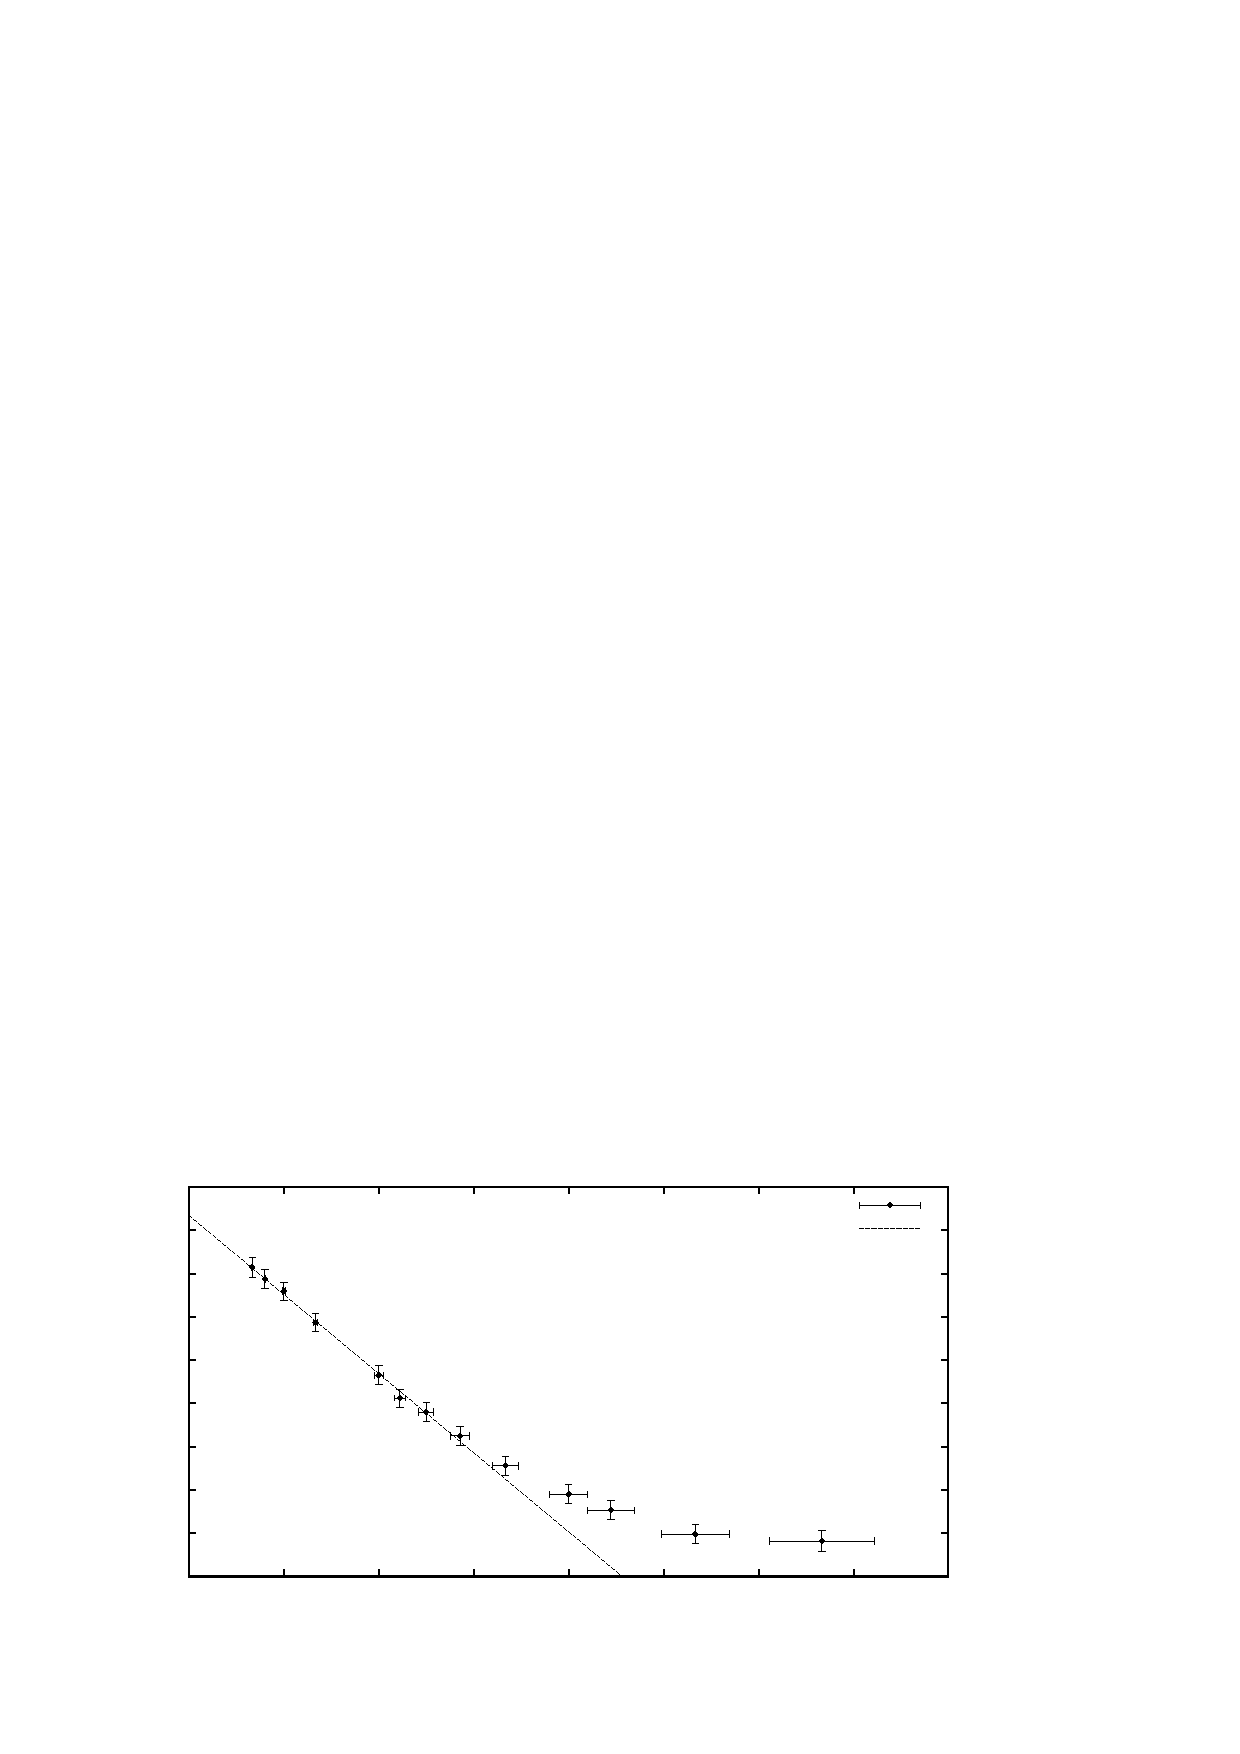
\includegraphics{diagram2}}%
    \gplfronttext
  \end{picture}%
\endgroup

	\end{figure}

\end{document}

